%%%%%%%%%%%%%%%%%%%%%%%%%%%%%%%%%%%%%%%%%%%%%%%%%%%%%%%%%%%%%%%%%%%%%%%%
% Escuela Politécnica Superior de la Universidad de Alicante
% Realizado por: Jose Manuel Requena Plens
% Contacto: info@jmrplens.com / Telegram:@jmrplens
%%%%%%%%%%%%%%%%%%%%%%%%%%%%%%%%%%%%%%%%%%%%%%%%%%%%%%%%%%%%%%%%%%%%%%%%

\definecolor{mycolor1}{rgb}{0.60000,0.00000,0.60000}%
%
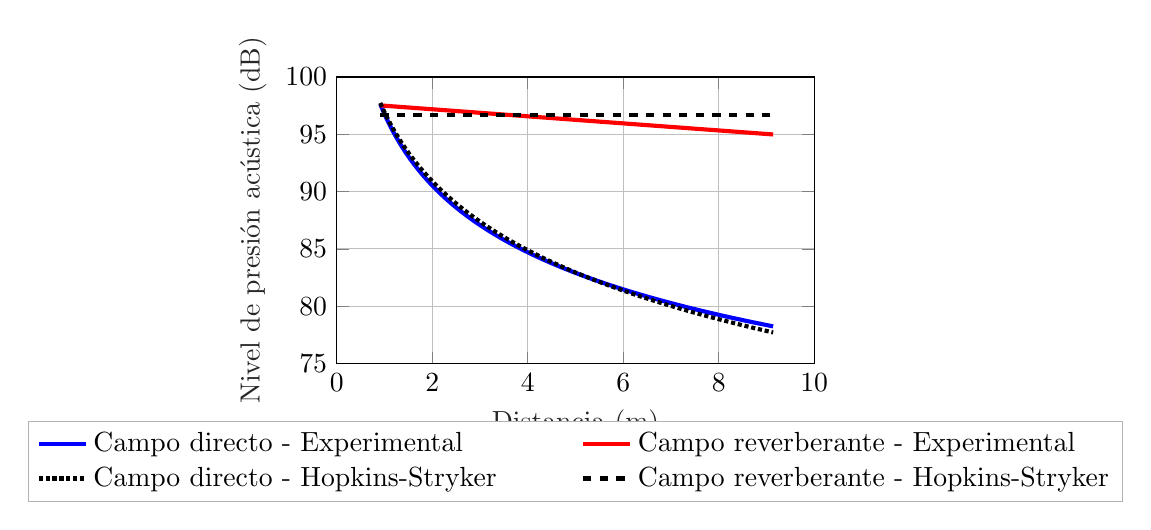
\begin{tikzpicture}

\begin{axis}[%
width=0.5\textwidth,
height=0.3\textwidth,
at={(0\textwidth,0\textwidth)},
scale only axis,
xmin=0,
xmax=10,
xlabel style={font=\color{white!15!black}},
xlabel={Distancia (m)},
ymin=75,
ymax=100,
ytick distance=5,
ylabel style={font=\color{white!15!black}},
ylabel={Nivel de presión acústica (dB)},
axis background/.style={fill=white},
xmajorgrids,
ymajorgrids,
legend style={at={(0.5,-0.03)}, anchor=north, legend cell align=left, align=left, draw=white!15!black},
legend columns = 2,legend style={at={(0.5,-0.2)}, anchor=north, legend cell align=left, align=left, draw=white!70!black, /tikz/every even column/.append style={column sep=1.0cm}}
]
\addplot [color=blue,line width=1.5pt]
  table[row sep=crcr]{%
0.911043357914437	97.6380061935451\\
0.971043357914425	97.0416130715755\\
1.03104335791443	96.484310473315\\
1.10104335791443	95.8774048250365\\
1.17104335791443	95.3113917575971\\
1.24104335791444	94.7813060660669\\
1.31104335791443	94.2830244776188\\
1.38104335791444	93.8130865478216\\
1.46104335791443	93.3069806543866\\
1.54104335791443	92.8303775474136\\
1.62104335791443	92.3801537924959\\
1.70104335791443	91.9536509875259\\
1.78104335791443	91.5485883526324\\
1.87104335791443	91.1160767261982\\
1.96104335791443	90.7057903345106\\
2.05104335791444	90.3156426154386\\
2.14104335791443	89.9438239896602\\
2.23104335791443	89.5887552104351\\
2.33104335791442	89.2121989170647\\
2.43104335791443	88.8529466109456\\
2.53104335791443	88.5095386461936\\
2.63104335791444	88.1806902279387\\
2.74104335791444	87.8344205548337\\
2.85104335791443	87.5030577659302\\
2.96104335791443	87.1854208783258\\
3.07104335791443	86.8804620884833\\
3.18104335791443	86.5872475992273\\
3.30104335791444	86.2797919676868\\
3.42104335791443	85.9843498413856\\
3.54104335791443	85.7000543544441\\
3.66104335791444	85.426127966722\\
3.79104335791443	85.1402654198586\\
3.92104335791443	84.8649508844128\\
4.05104335791444	84.5994642356986\\
4.18104335791443	84.3431556826281\\
4.32104335791443	84.0767218124595\\
4.46104335791443	83.8195859804349\\
4.60104335791443	83.5711467621151\\
4.75104335791443	83.3139935284142\\
4.90104335791443	83.0655890600581\\
5.05104335791444	82.8253812483105\\
5.20104335791443	82.5928679479935\\
5.36104335791443	82.3528195444158\\
5.52104335791444	82.120498287441\\
5.68104335791443	81.8954420472253\\
5.85104335791443	81.6638082159739\\
6.02104335791444	81.4394362677818\\
6.19104335791442	81.2219029078978\\
6.37104335791443	80.9985968064552\\
6.55104335791444	80.7821012050116\\
6.74104335791444	80.5605400646246\\
6.93104335791443	80.3457203545647\\
7.12104335791443	80.1372603842554\\
7.32104335791443	79.9243144622446\\
7.52104335791444	79.7176514144308\\
7.73104335791443	79.5070397973059\\
7.94104335791442	79.3026073677421\\
8.15104335791443	79.1040164504568\\
8.37104335791443	78.9018955433603\\
8.59104335791443	78.7055148221739\\
8.82104335791443	78.5060156380693\\
9.05104335791444	78.3121381646318\\
9.14104335791443	78.2377385102596\\
};
\addlegendentry{Campo directo - Experimental}

\addplot [color=red,line width=1.5pt]
  table[row sep=crcr]{%
0.911043357914437	97.5218752230605\\
9.14104335791443	94.9864450736265\\
};
\addlegendentry{Campo reverberante - Experimental}

\addplot [color=black, densely dotted, line width=1.5pt]
  table[row sep=crcr]{%
0.911043357914437	97.7331926631792\\
0.971043357914425	97.1792011477379\\
1.04104335791443	96.5745972347531\\
1.11104335791443	96.0093534389856\\
1.18104335791443	95.4786567564759\\
1.25104335791443	94.9785263574731\\
1.33104335791442	94.4401295353534\\
1.41104335791444	93.9331664115882\\
1.49104335791444	93.4541681380115\\
1.57104335791443	93.0002101682137\\
1.65104335791443	92.5688040192524\\
1.74104335791444	92.1077818536397\\
1.83104335791442	91.67000102226\\
1.92104335791443	91.253230247119\\
2.01104335791443	90.8555449059847\\
2.11104335791443	90.4340305227801\\
2.21104335791443	90.0320284059368\\
2.31104335791443	89.6478117182375\\
2.41104335791444	89.2798731791945\\
2.52104335791444	88.892367288714\\
2.63104335791444	88.5214134861318\\
2.74104335791444	88.1656554813739\\
2.85104335791443	87.8238971470306\\
2.97104335791443	87.4657937924312\\
3.09104335791443	87.121871648269\\
3.21104335791443	86.7910501914252\\
3.33104335791442	86.4723678740925\\
3.46104335791443	86.1398327886619\\
3.59104335791443	85.8195606111837\\
3.72104335791443	85.5106789771931\\
3.85104335791443	85.2124054217199\\
3.99104335791444	84.9022446689407\\
4.13104335791444	84.602778523021\\
4.27104335791444	84.3132939822976\\
4.41104335791444	84.033147053859\\
4.56104335791443	83.7426895724501\\
4.71104335791443	83.4616315615413\\
4.86104335791443	83.1893836916001\\
5.02104335791444	82.9080941543875\\
5.18104335791443	82.635629052434\\
5.34104335791443	82.3714515163175\\
5.51104335791443	82.0992970302704\\
5.68104335791443	81.8354115101393\\
5.85104335791443	81.5793072595462\\
6.03104335791443	81.3161245733647\\
6.21104335791443	81.0606823675505\\
6.39104335791443	80.8125383092309\\
6.58104335791442	80.5580785454699\\
6.77104335791444	80.3108616913113\\
6.96104335791443	80.0704868101745\\
7.16104335791444	79.8244475218628\\
7.36104335791443	79.585186070651\\
7.57104335791443	79.3408589206871\\
7.78104335791443	79.1032168805553\\
7.99104335791444	78.8719038454604\\
8.21104335791443	78.6360066789118\\
8.43104335791443	78.4063471322951\\
8.66104335791444	78.1725693325264\\
8.89104335791443	77.9449190244605\\
9.13104335791444	77.7135654870847\\
9.14104335791443	77.704058208972\\
};
\addlegendentry{Campo directo - Hopkins-Stryker}

\addplot [color=black, dashed, line width=1.5pt]
  table[row sep=crcr]{%
0.911043357914437	96.7131831634935\\
9.14104335791443	96.7131831634935\\
};
\addlegendentry{Campo reverberante - Hopkins-Stryker}



\end{axis}
\end{tikzpicture}%